\documentclass[conference]{IEEEtran}
\IEEEoverridecommandlockouts
% The preceding line is only needed to identify funding in the first footnote. If that is unneeded, please comment it out.
\usepackage{cite}
\usepackage{amsmath,amssymb,amsfonts}
\usepackage{algorithmic}
\usepackage{graphicx}
\usepackage{textcomp}
\usepackage{xcolor}
\usepackage{tabularx}
\usepackage{multirow}
\usepackage{graphics} % for pdf, bitmapped graphics files
\usepackage{subfig}
\usepackage{subcaption}
\usepackage{hyperref}
\usepackage{academicons}
\usepackage{xcolor}
\usepackage{listings}
\usepackage{tabularx} % Asegúrate de incluir este paquete

\usepackage{tikz}
\usetikzlibrary{shapes.geometric, arrows}

\usetikzlibrary{shapes.geometric, arrows}

\tikzstyle{startstop} = [rectangle, rounded corners, minimum width=3cm, minimum height=1cm,text centered, draw=black, fill=red!30]
\tikzstyle{process} = [rectangle, minimum width=3cm, minimum height=1cm, text centered, draw=black, fill=blue!30]
\tikzstyle{arrow} = [thick,->,>=stealth]


\def\BibTeX{{\rm B\kern-.05em{\sc i\kern-.025em b}\kern-.08em
		T\kern-.1667em\lower.7ex\hbox{E}\kern-.125emX}}

% Color Enlace
\definecolor{colorEnlace}{RGB}{0, 0, 0}
\hypersetup{
	colorlinks=true,
	linkcolor=colorEnlace,
	citecolor=colorEnlace,
	urlcolor=colorEnlace,
	pdfauthor={Davis Bremdow Salazar Roa},
	pdftitle={Sistemas Embebidos}
}
\definecolor{mybg}{rgb}{0.97,0.97,0.97}
\definecolor{mygray}{gray}{0.4}
\definecolor{mygreen}{rgb}{0,0.6,0}
\definecolor{myblue}{rgb}{0,0,0.8}
\definecolor{mypurple}{rgb}{0.58,0,0.82}
\definecolor{myred}{rgb}{0.7,0,0}

\lstdefinelanguage{MatlabEnhanced}{
	language=Matlab,
	morekeywords={[2]linspace,plot,title,xlabel,ylabel,legend,grid},
	morekeywords={[3]sin,cos,exp,log,sqrt},
	keywordstyle=\color{myblue}\bfseries,
	keywordstyle=[2]\color{mypurple},
	keywordstyle=[3]\color{myred},
	commentstyle=\color{mygreen}\itshape,
	stringstyle=\color{mygray},
	morecomment=[l]%
}

\lstset{
	language=MatlabEnhanced,
	backgroundcolor=\color{mybg},
	frame=single,
	basicstyle=\ttfamily\small,
	showstringspaces=false,
	numbers=none,              %
	xleftmargin=0pt,           %
	framexleftmargin=0pt,      
	framexrightmargin=0pt,
	framextopmargin=2pt,
	framexbottommargin=2pt,
	breaklines=true,
	tabsize=1,
}

% Control 
\usepackage{amsmath}
\begin{document}
	
	\title{Informe final - Amplificador Diferencial Retroalimentado}
	\author{
		\makebox[\textwidth][c]{\large\textbf{Universidad Nacional de San Antonio Abad del Cusco}}\\
		\makebox[\textwidth][c]{\normalsize\textit{Escuela profesional de Ingeniería Electrónica}}\\
		\makebox[\textwidth][c]{\normalsize\textit{Laboratorio de Circuitos Electrónicos III}}\\
		\and
		\centering
		\IEEEauthorblockN{Ing. Milton Velasquez Curo}
		\IEEEauthorblockA{Ingeniero Electrónico \\
			Cusco, Perú \\
			milton.velasquez@unsaac.edu.pe}
		\and
		\IEEEauthorblockN{Davis Bremdow Salazar Roa - 200353}
		\IEEEauthorblockA{Estudiante de Ingeniería Electrónica \\
			Cusco, Perú \\
			200353@unsaac.edu.pe}
	}
	
	\maketitle
	\begin{abstract}
		La modulación es un proceso fundamental en las telecomunicaciones que consiste en variar una o más propiedades de una señal portadora (como amplitud, frecuencia o fase) en función de una señal de información o mensaje. Este proceso permite transmitir información a largas distancias de manera eficiente, minimizando interferencias y aprovechando mejor el espectro de frecuencias. Existen varios tipos de modulación, entre ellos la modulación en amplitud (AM), frecuencia (FM) y fase (PM), cada una con características y usos específicos según las necesidades del sistema de comunicación.
		
		El índice de modulación es una medida que cuantifica la variación de la señal portadora en relación con la señal moduladora. Su importancia radica en que determina la eficiencia espectral, la calidad de la señal transmitida y el nivel de distorsión. Un índice bajo puede resultar en una señal débil o difícil de demodular, mientras que un índice muy alto puede causar sobre modulación y distorsión. En aplicaciones prácticas, la modulación es utilizada en radiodifusión (radio y televisión), comunicaciones satelitales, telefonía móvil, redes Wi-Fi, y sistemas de control industrial, donde el índice de modulación debe ser cuidadosamente ajustado para garantizar un rendimiento óptimo.
	\end{abstract}
	
	\begin{IEEEkeywords}
		Modulación, portadora, señal, índice de modulación, amplitud, frecuencia, fase, transmisión, espectro, distorsión.
	\end{IEEEkeywords}
	%% Contenido del documento
	\section{Modulación AM con portadora (Radio AM) - DSB - LC}
	
	\section{Modulación AM sin Portadora - DSB - SC para transmisión de TV Analógica}
	\subsection{Expresión de la señal modulada}
	\begin{align*}
		m(t) &= 2\cos(2\pi \cdot 1000t) + \cos(2\pi \cdot 3000t) \\
		c(t) &= 10\cos(2\pi \cdot 100\,000t) \\
		\varphi(t) &= m(t) \cdot 10 \cos(2\pi \cdot 100\,000t) \\
		\varphi(t) &= \left[2\cos(2\pi \cdot 1000t) + \cos(2\pi \cdot 3000t)\right] \cdot 10 \cos(2\pi \cdot 100\,000t) \\
		\varphi(t) &= 20 \cos(2\pi \cdot 1000t) \cos(2\pi \cdot 100\,000t) + 10 \cos(2\pi \cdot 3000t) \cos(2\pi \cdot 100\,000t) \\
		\varphi(t) &= 10 \cos(2\pi \cdot 101\,000t) + 10 \cos(2\pi \cdot 99\,000t) + 5 \cos(2\pi \cdot 103\,000t) + 5 \cos(2\pi \cdot 97\,000t) \\
	\end{align*}
	\subsection{Compare la potencia transmitida con el caso de AM convencional}
	\begin{align*}
		P_T &= \frac{10^2}{2} + \frac{5^2}{2} \\
		P_T &= 125 [W]
	\end{align*}
	
	Debido a que este tipo de modulación no cuenta con una portadora para su transmisión la potencia a usar es menor
	\subsection{Analice el espectro y discuta las ventajas de DSB-SC en transmisión de video analogica respecto a AM con portadora}
	
	El espectro de la señal se desplazara en función de la frecuencia de la portadora como se muestra en la figura \ref{fig:dbs-sc-espectro}
	\begin{figure}[h]
		\centering
		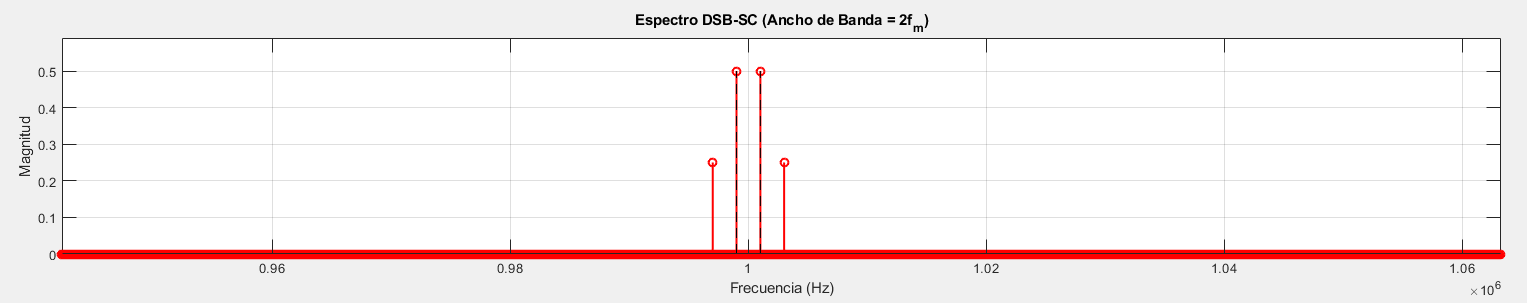
\includegraphics[width=0.5\textwidth]{media/dbs-sc-espectro}
		\caption{Espectro de la señal - DSB - SC}
		\label{fig:dbs-sc-espectro}
	\end{figure}
	
	La modulación DSB-SC (Double Sideband Suppressed Carrier) Al suprimir la portadora, DSB-SC reduce la potencia necesaria para la transmisión, permitiendo que toda la energía se concentre en las bandas laterales que contienen la información incrementando la eficiencia en la transmisión lo cual es de vital importancia para la transmisión de video.
	
	\subsection{Implemente una simulación en MATLAB que incluya la demodulación coherente}
	Para realizar esta demodulación es necesario volver a multiplicar la portadora a la señal AM modulada y para lo cual en el código de matlab se definieron las siguientes lineas para realizar este proceso.
	
	\begin{lstlisting}[caption={}, numbers=none]
		clc; clear; close all;
		fs = 10000000;                 % Frecuencia de muestreo
		t = 0:1/fs:0.1-1/fs;         % Vector de tiempo (100 ms)
		N = length(t);               % Numero de muestras
		
		%% PARAMETROS DE SENALES
		% Portadora
		fc = 1000000;                   % Frecuencia portadora
		Ac = 1;                      % Amplitud portadora
		
		% Moduladora (mensaje)
		fm = 1000;                    % Frecuencia mensaje
		Am = 2;                      % Amplitud mensaje
		% m = Am*cos(2*pi*fm*t);       % Senal moduladora
		m = Am*(cos(2*pi*fm*t) + (1/2)*cos(2*pi*3*fm*t) );       % Senal moduladora
		% Portadora
		c = Ac*cos(2*pi*fc*t);
		
		% DSB-SC
		dsb_sc = m .* c;
		
		demodulacion = dsb_sc.*c;
		
		% Espectro de la senal demodulada
		demo_frecuencia = abs(fftshift(fft(demodulacion)/N));
		
		%Mostrar el resultado
		figure;
		plot(t, demodulacion); 
		figure;
		plot(f, demo_frecuencia);
	\end{lstlisting}
	
	Siendo el resultado el que se aprecia en la figura \ref{fig:demo-dsb-sc-tiempo} y \ref{fig:demo-dsb-sc-frecuencia} para el tiempo y la frecuencia respectivamente
	
	\begin{figure}[h]
		\centering
		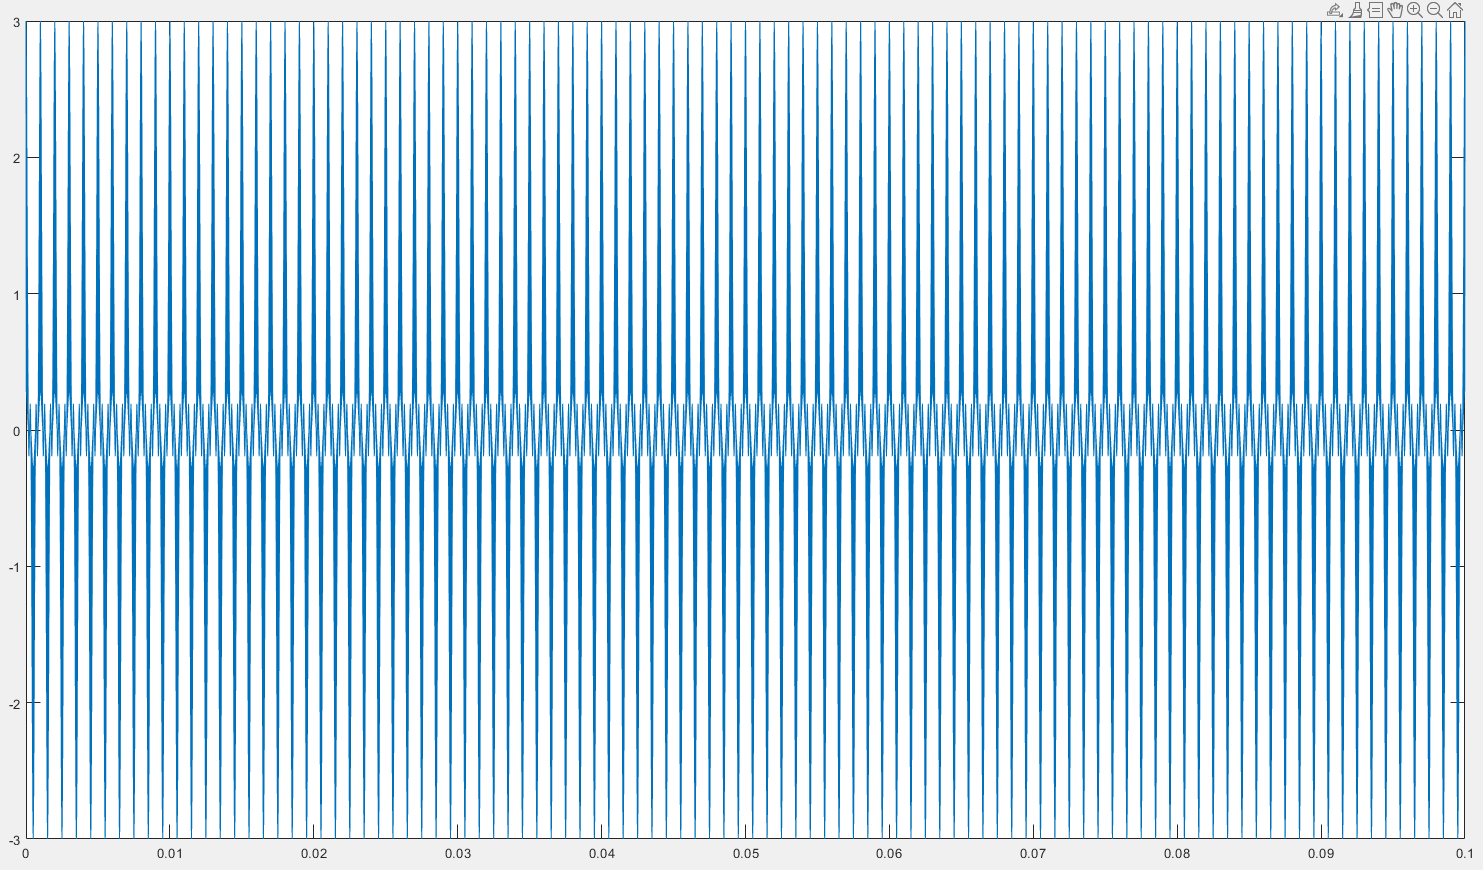
\includegraphics[width=0.5\linewidth]{media/demo-dsb-sc-tiempo}
		\caption{Demodulación en tiempo - DSB - SC}
		\label{fig:demo-dsb-sc-tiempo}
	\end{figure}
	
	\begin{figure}[h]
		\centering
		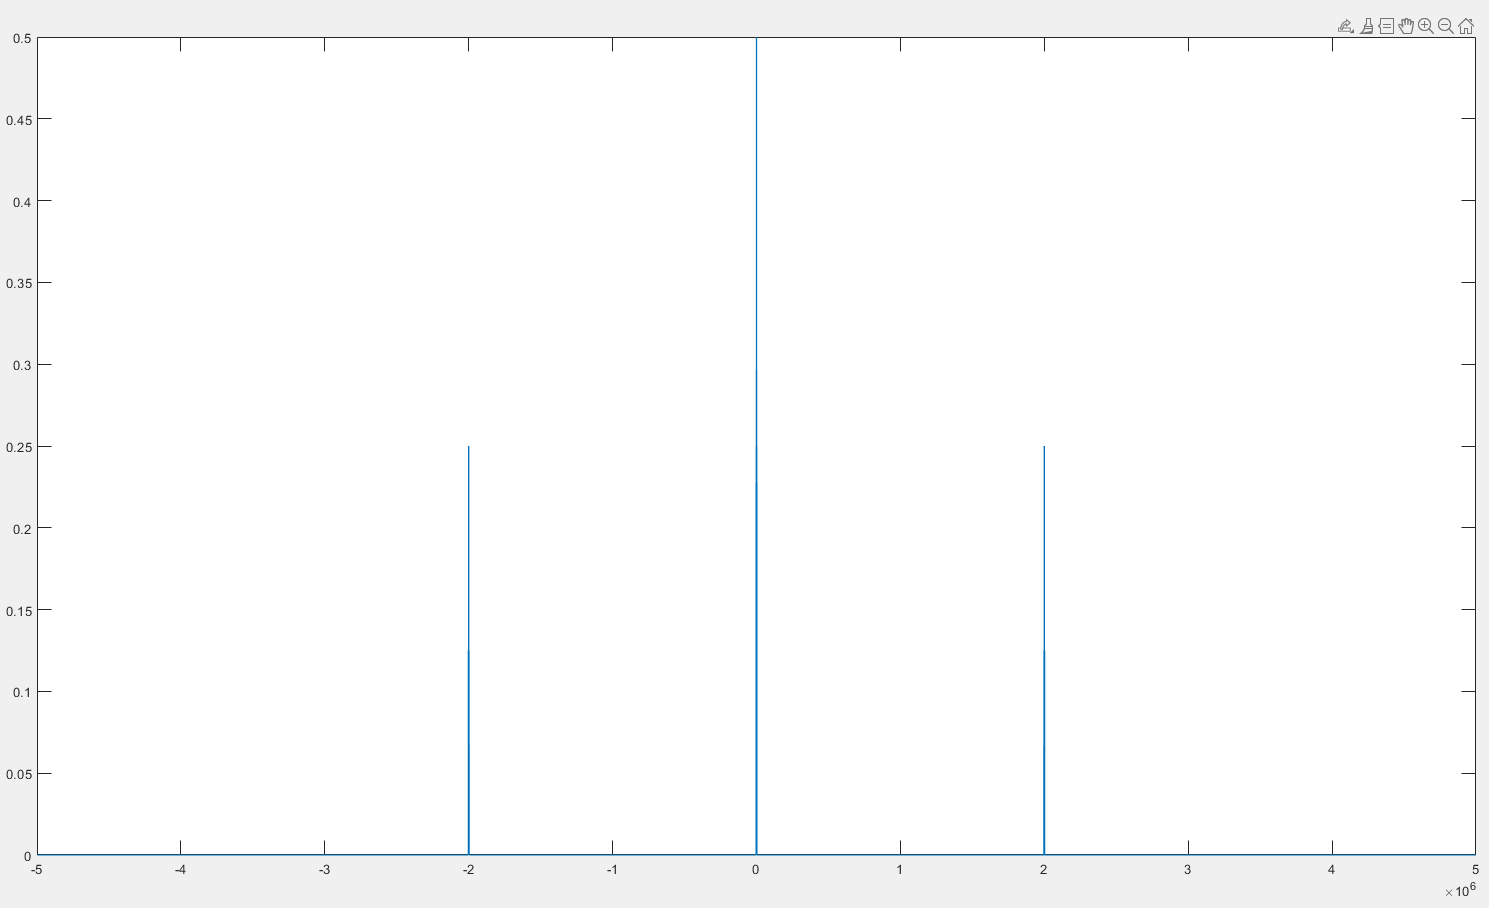
\includegraphics[width=0.5\linewidth]{media/demo-dsb-sc-frecuencia}
		\caption{Demodulación - frecuencia}
		\label{fig:demo-dsb-sc-frecuencia}
	\end{figure}
	
	
	\section{Mencione que precauciones se deben tener en la sincronización entretransmisor y receptor en este tipo de modulación}
	
	En la modulación DSB-SC, una de las principales precauciones que se debe tener es la correcta sincronización entre el transmisor y el receptor, ya que la portadora es suprimida y no se transmite junto con la señal modulada. Esto implica que el receptor debe generar una portadora local que tenga la misma frecuencia y fase que la original para poder demodular correctamente la señal
	
	Siendo así que una desincronización en frecuencia produce distorsión en la señal recuperada, mientras que un desfase genera atenuación o inversión de la información. Viendo como necesidad una correcta sincronización entre estos dispositivos.
	
	\section{Banda Lateral Única SSB en comunicación HF}
	
	\subsection{Derive la expresion para la modulación USB (Upper Side Band)}
	\begin{align*}
		c(t) &= 10 \cos(2\pi \cdot 100\,\text{k} t), \\
		m(t) &= 3 \cos(2\pi \cdot 2000t) = 2 \sin(2\pi \cdot 4000t), \\
		\varphi(t) &= m(t) \cdot 10 \cos(2\pi \cdot 100\,\text{k} t), \\
		\varphi(t) &= 3 \cos(2\pi \cdot 2000t) \cdot 10 \cos(2\pi \cdot 100\,\text{k} t) 
		= 20 \sin(2\pi \cdot 4000t) \cos(2\pi \cdot 100\,\text{k} t), \\
		\varphi(t) &= 15 \cos(2\pi \cdot 102\,\text{k} t) + 15 \cos(2\pi \cdot 98\,\text{k} t) 
		- 10 \sin(2\pi \cdot 104\,\text{k} t) + 10 \sin(2\pi \cdot 96\,\text{k} t), \\
		\text{Luego del filtro se tendrá:} \\
		\varphi(t) &= 15 \cos(2\pi \cdot 102\,\text{k} t) - 10 \sin(2\pi \cdot 104\,\text{k} t)
	\end{align*}
	\subsection{Calcule el ancho de banda ocupado comparado con AM convencional y DSB.}
	\textbf{Ancho de banda (BW):}
	\begin{align*}
		\text{SSB:} &\quad \text{BW} = W_m \\
		\text{DSB-SC:} &\quad \text{BW} = 2W_m \\
		\text{DSB-LC:} &\quad \text{BW} = 2W_m \\
		&\quad \text{BW} = 2\pi W_m \\
		&\quad \text{BW} = 2\pi \cdot 4000 \\
		&\quad \text{BW} = 8000\pi
	\end{align*}
	\subsection{Implemente en MATLAB el método de filtrado para obtener SSB.}
	
	\begin{figure}[h]
		\centering
		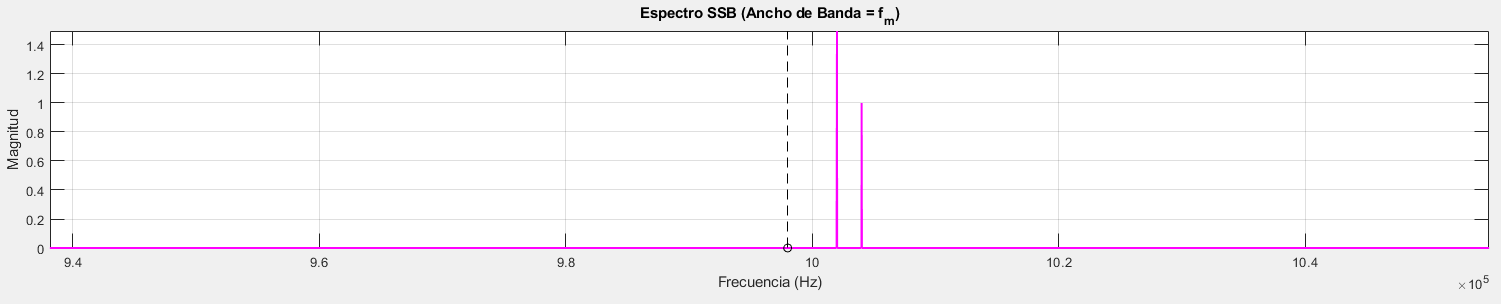
\includegraphics[width=0.4\linewidth]{media/ssb-usb}
		\caption{Señal SSB - USB}
		\label{fig:ssb-usb}
	\end{figure}
	\begin{lstlisting}[numbers=none]
		%% CONFIGURACION INICIAL
		clc; clear; close all;
		fs = 10000000;                 % Frecuencia de muestreo
		t = 0:1/fs:0.1-1/fs;         % Vector de tiempo (100 ms)
		N = length(t);               % Numero de muestras
		
		%% PARAMETROS DE SENALES
		% Portadora
		fc = 1000000;                   % Frecuencia portadora
		Ac = 1;                      % Amplitud portadora
		
		% Moduladora (mensaje)
		fm = 2000;                    % Frecuencia mensaje
		Am = 3;                      % Amplitud mensaje
		% m = Am*cos(2*pi*fm*t);       % Senal moduladora
		m = Am*cos(2*pi*fm*t) - 2*sin(2*pi*2*fm*t);       % Senal moduladora
		
		%% GENERACION DE SENALES
		% Portadora
		c = Ac*cos(2*pi*fc*t);
		
		% DSB-SC
		dsb_sc = m .* c;
		
		% SSB (Metodo de filtrado)
		filtro_pb = fir1(100, 1100/(fs/2), 'high');  % Filtro pasa bajos
		hilbert_m = imag(hilbert(m));   % Transformada de Hilbert
		ssb_usb = (m.*cos(2*pi*fc*t) - (hilbert_m.*sin(2*pi*fc*t)));
		ssb_usb = filter(filtro_pb, 1, ssb_usb); % Filtrado final
	\end{lstlisting}
	
	
	\subsection{Comente por que SSB es ampliamente usada en comunicaciones maritimas, aeronauticas y de radioaficionados en Perú}
	La modulación SSB (Single Sideband) es ampliamente utilizada en comunicaciones marítimas, aeronáuticas y de radioaficionados en Perú debido a su alta eficiencia en el uso del espectro y la potencia, lo que permite transmisiones de largo alcance con equipos de baja potencia, ideales para entornos donde los recursos son limitados o las distancias son extensas. Al transmitir solo una de las bandas laterales y suprimir la portadora, SSB reduce el ancho de banda necesario y mejora la relación señal/ruido, lo cual es crucial en zonas rurales, selvas o regiones costeras peruanas donde las condiciones de propagación pueden ser adversas y los enlaces confiables son vitales para la seguridad y la coordinación operativa.
	
		
	\bibliographystyle{IEEEtran}
	\bibliography{biblio}
\end{document}
